% !TeX root=main.tex

\chapter{مفاهیم پایه} \label{ch:basics}
\thispagestyle{empty}


\section{مقدمه}
\paragraph{}
{
    در این بخش به معرفی مفاهیم پایه درباره سکوی کوبرنیتز، پروژه کوبلت مجازی، اینترنت اشیاء و برخی معماری‌هایی که 
    در این پروژه استفاده شده‌اند به مانند 
    استخر کارگران\footnote{\lr{Worker Pool}}
    پرداخته‌شده است.
}

\section{بستر ابری}
\label{sec:cloudenv}
\paragraph{}
{
    بستر ابری\footnote{\lr{Cloud Environment}}
    به محیطی اشاره دارد که منابع محاسباتی، شبکه و ذخیره سازی را برای ارائه خدمات به صورت ابری و توسط یک ارائه دهنده ابری فراهم می کند.
    در این محیط، خدمات و برنامه‌ها بر روی سرورهای فیزیکی مجازی‌سازی شده قرار می گیرند و کاربران می توانند به آنها از طریق اینترنت وصل شوند
    و از آنها استفاده کنند. با استفاده از محیط ابری، امکاناتی مانند انعطاف پذیری بالا، قابلیت مقیاس‌پذیری، اشتراک گذاری منابع و مدیریت
    آسانتر برای خدمات فراهم می شود. همچنین یکی از مزیت‌های بستر ابری ساده سازی ساخت، مدریت و انتشار یک خدمت می‌باشد.
}

\section{سکوی کوبرنیتز}
\label{sec:kubernetes}
\paragraph{}
{
    کوبرنیتز\footnote{\lr{Kubernetes}}
    یک سامانه مدیریت
    کانتینرها\footnote{\lr{Containers}}
    است که توسط گوگل توسعه داده شده است و در حال حاضر تحت نظارت و پشتیبانی مؤسسه
    CNCF\footnote{\lr{Cloud Native Computing Foundation}}
    قرار دارد. این ابزار به توسعه‌دهندگان و مدیران سامانه امکان می‌دهد برنامه‌ها و خدمات را در
    بسترهای ابری\footnote{\lr{Cloud Environment}}
    مدیریت کنند و کانتینرها را به طور موثر و مقیاس‌پذیر در
    محیط‌های توزیع شده\footnote{\lr{Distributed Environment}}
    مدیریت کنند.
    
    از طریق کوبرنیتز، می‌توان کانتینرها را بر روی یک
    سرور مجازی\footnote{\lr{Virtual Machine}}
    یا 
    فیزیکی\footnote{\lr{Physical Server}}
    اجرا کرده و مدیریت آنها را ساده‌تر و مؤثرتر نمود. این سامانه با بهره‌گیری از روش‌هایی مانند
    اتوماسیون\footnote{\lr{automation}}
    ، توازن بار\footnote{\lr{Load Balancing}}
    و تشخیص خودکار اشکال\footnote{\lr{Automatic Diagnostics}}
    ، مدیریت و کنترل بهبود یافته‌ای در محیط‌های مبتنی بر کانتینر فراهم می‌کند.
    این ابزار برای حل مشکلات زیر موثر است:
    \begin{enumerate}
        \item مقیاس‌پذیری: کوبرنیتز می‌تواند تعداد کانتینرها و پیش‌نمونه‌های برنامه را بر اساس نیازهای ترافیک و خدمت تنظیم کند. با استفاده از مدیریت منابع مبتنی بر درخواست، میزان منابع مورد استفاده توسط برنامه را به طور خودکار تنظیم می‌کند و مقیاس‌پذیری عمودی و افقی را به راحتی فراهم می‌کند.
        \item توازن بار: با استفاده از کوبرنیتز، می‌توان بار کار را به طور متوازن بین نودها و سرورهای مختلف تقسیم کرد. این باعث بهبود عملکرد و عدم وقوع اختلال در سامانه می‌شود. همچنین، در صورتی که یک نود یا سرور دچار مشکل شود، کوبرنیتز به طور خودکار کار را به سایر نودها منتقل می‌کند.
        \item مدیریت پیچیدگی: کوبرنیتز امکاناتی را برای مدیریت پیچیدگی سامانه‌های کانتینری فراهم می‌کند. این ابزار اجرا، مدیریت، نظارت و زندگی‌دوباره سازی کانتینرها را ساده می‌کند. همچنین امکاناتی برای مدیریت تنظیمات، آپدیت‌ها، و تغییرات در حال اجرا نیز در اختیار کاربران قرار می‌دهد.
        \item قابلیت انتقال: کوبرنیتز امکان انتقال برنامه‌ها و خدمات بین بسترهای مختلف را فراهم می‌کند. با استفاده از این امکان، می‌توان برنامه‌ها را بین محیط‌های توسعه، آزمون و تولید به راحتی منتقل کرد. کوبرنیتز با استفاده از این قابلیت‌ها و خصوصیات، به توسعه‌دهندگان و مدیران سامانه امکان می‌دهد برنامه‌ها را به صورت مؤثر، قابلیت مقیاس‌پذیری و قابل اطمینان در محیط‌های کانتینری مدیریت کنند و عملکرد سامانه را بهبود دهند.
    \end{enumerate}
    \begin{figure}[H]
        \center{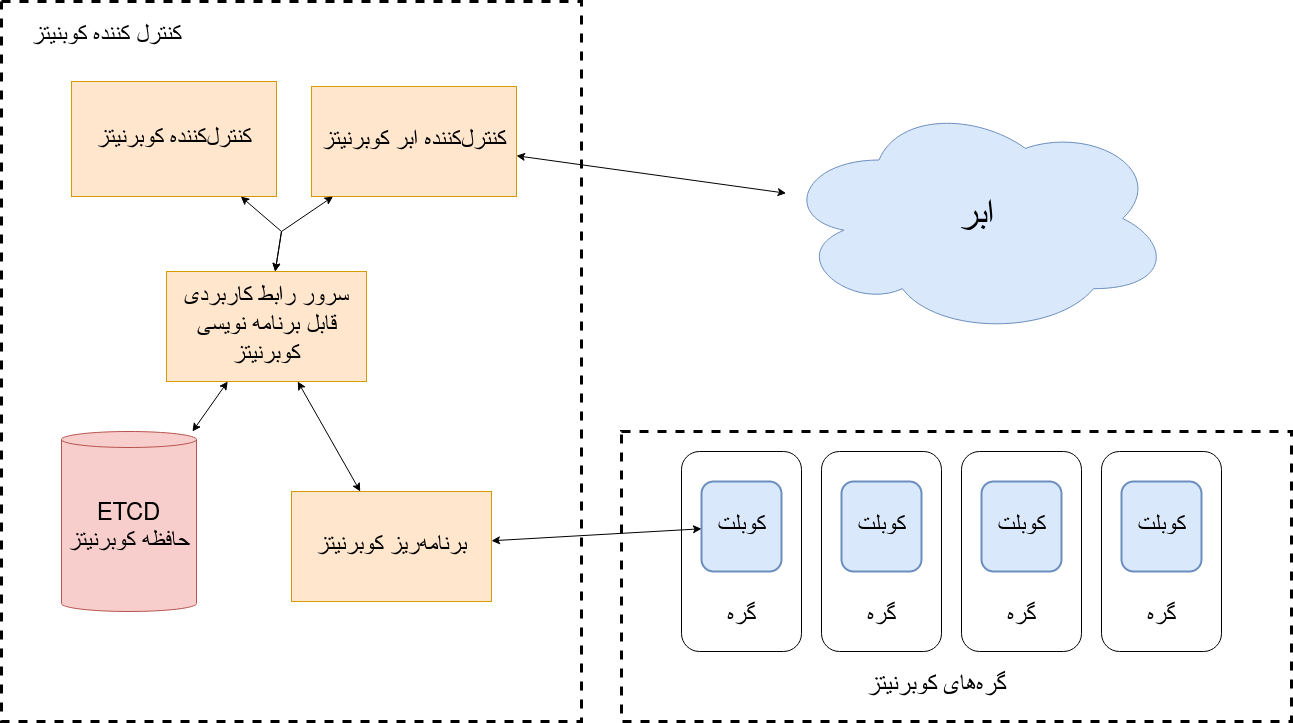
\includegraphics[width=\textwidth]{figs/kube_compontents.png}}
        \caption{معماری کلی کوبرنیتز}
        \label{fig:kube_compontents}
    \end{figure}
}

\subsection{کانتینر‌}
\label{subsec:containers}
\paragraph{}
{
    کانتینرها یک فناوری پیشرفته در زمینه مدیریت و اجرای نرم‌افزار هستند. یک کانتینر، یک واحد نرم‌افزاری است که تمام نیازمندی‌های
    لازم برای اجرای یک نرم‌افزار را شامل می‌شود. در واقع، کانتینرها مجموعه‌ای از عملیات سامانه‌ای، کدها و تنظیماتی هستند که با 
    یکدیگر در یک بستر محصور می‌شوند. از ویژگی‌های برجسته کانتینرها،می‌توان به استقلال و حمل‌پذیری آن‌ها اشاره کرد. به عبارتی دیگر،
    یک کانتینر می‌تواند بدون تغییر و با حفظ کارایی خود، بین بستر‌ها و سامانه‌‌های عامل‌ منتقل شود. این ویژگی باعث شده است که کانتینرها
    در صنعت فناوری اطلاعات بسیار محبوب شوند. برای مدیریت کانتینرها، ابزارهای مختلفی وجود دارند. یکی از محبوب‌ترین ابزارها برای مدیریت کانتینرها،
    داکر\footnote{\lr{Docker}}
    است. داکر یک بستر توسعه نرم‌افزار مبتنی بر کانتینر است که به توسعه‌دهندگان امکان می‌دهد تا برنامه‌های خود را در یک کانتینر قرار داده و آن را در
    هر سامانه‌ای اجرا کنند. با استفاده از کانتینرها، عملیات توسعه، آزمون و استقرار نرم‌افزارها سریع‌تر و ساده‌تر می‌شود. با توجه به این که هر کانتینر
    دارای محیط مستقلی است، احتمال بروز تداخل بین برنامه‌ها به حداقل می‌رسد و تغییرات در یک کانتینر بر روی سایر کانتینرها تأثیری نمی‌گذارد. همچنین،
    سبک بودن کانتینرها امکان مقیاس‌پذیری بالایی را فراهم می‌آورد.
}

\subsection{پاد}
\label{subsec:pod}
\paragraph{}
{
    پاد‌ها\footnote{\lr{پادs}} در کوبنیتز واحد اصلی اجرا و مدیریت برنامه‌ها و خدمات هستند. یک پاد شامل یک یا چند کانتینر مرتبط است که به صورت مشترک منابع شبکه و ذخیره‌سازی را به اشتراک می‌گذارند. همچنین، هر پاد دارای یک آدرس یکتا درون کلاستر است. پاد‌ها به صورت لایه‌ای مجازی شبیه سازی می‌شوند و انتزاعی از یک ماشین مجازی یا سامانه عامل فیزیکی هستند. این انتزاع به برنامه‌ها امکان می‌دهد تا بدون احتیاج به اطلاعات جزئیات بستری که برای اون اجرا می‌شوند، در محیط کنترلی کوبرنیتز اجرا شوند. بنابراین، پاد‌ها برای توسعه‌دهندگان و مدیران سامانه، یک واسط سطح بالا و یک فضای کاری است.
}

\subsection{گره}
\label{subsec:node}
\paragraph{}
{
    در بستر کوبنیتز، گره‌ها\footnote{\lr{Node}} از اجزای کلیدی هستند که برنامه‌ها و خدمات در آن‌ها اجرا می‌شوند. یک گره 
    معمولاً یک سرور فیزیکی یا ماشین مجازی است که بر روی آن کانتینرها اجرا می‌شوند. هر گره شامل عناصر زیر است:
    \begin{enumerate}
        \item پلتفرم سخت‌افزاری: این شامل سرورها، سامانه‌های فیزیکی، یا ماشین‌های مجازی است که منابع سخت‌افزاری مانند پردازنده، حافظه، و دیسک را فراهم می‌کنند. گره‌ها بسته به نیازهای برنامه‌ها و خدمات، می‌توانند از طریق شبکه به یکدیگر متصل شوند.
        \item کوبلت\footnote{\lr{Kublet}}: مسئول مدیریت و اجرای کانتینرها در گره است. آن بر روی هر گره نصب شده و با کنترل کننده‌های کوبرنیتز برای دریافت توصیف کانتینرها و مدیریت آن‌ها در ارتباط است.
        \item پروکسی\footnote{\lr{Kube-proxy}}: یک کنترل کننده شبکه است که مسئول مدیریت ترافیک شبکه بین کانتینرها در گره است. این عملکرد به ارتباط و مسیریابی درخواست‌ها بین کانتینرها و اجزای دیگر کوبرنیتز مرتبط است.
        \item حافظه مشترک\footnote{\lr{Shared Memory}}: گره‌ها از یک حافظه مشترک برای ذخیره و به اشتراک گذاری اطلاعاتی مانند پیکربندی‌ها و وضعیت گره‌ها استفاده می‌کنند. این حافظه مشترک معمولاً از طریق ابزارهای ذخیره‌سازی مانند ETCD پیاده‌سازی می‌شود.
    \end{enumerate}
    با استفاده از گره‌ها، کوبرنیتز قادر است برنامه‌ها و خدمات را بر روی یک سری از سرورها یا ماشین‌های مجازی توزیع کند و به طور همزمان و مقیاس‌پذیر اجرا کند. این باعث افزایش انعطاف‌پذیری، بهره‌وری و پایداری در محیط‌های ابری و مجازی می‌شود.
}

\subsection{کوبلت}
\label{subsec:kubelet}
\paragraph{}
{
    کوبلت
    یکی از اجزای اصلی سامانه مدیریت کانتینرها کوبرنیتز است. کوبلت مسئول اجرا و مدیریت کانتینرها در یک
    گره
    می‌باشد. کوبلت در هر گره از
    خوشه\footnote{\lr{Cluster}}
    کوبرنیتز نصب شده و وظیفه‌ای اساسی را بر عهده دارد که شامل موارد زیر است:
    \begin{enumerate}
        \item مدیریت کانتینرها: کوبلت مسئول ساخت و اجرای کانتینرها بر اساس توصیف‌هایی که از طرف کنترل کننده‌های کوبرنیتز به آن ارسال می‌شود، می‌باشد. این توصیف‌ها شامل اطلاعاتی مانند نرم‌افزار مورد نظر، تنظیمات شبکه و منابع مصرفی کانتینر می‌شوند.
        \item پایش\footnote{\lr{Monitoring}}منابع: کوبلت مسئول نظارت بر منابع مصرفی کانتینرها است و اطلاعات مربوط به استفاده از پردازنده، حافظه، شبکه و دیگر منابع سامانه را جمع‌آوری کرده و گزارش می‌دهد. این اطلاعات به کنترل کننده‌های کوبرنیتز ارسال می‌شوند تا بتوانند به‌طور هوشمند منابع را تخصیص دهند و بهینه‌سازی منابع را انجام دهند.
        \item بروزرسانی و نگهداری کانتینرها: کوبلت مسئول بروزرسانی و نگهداری کانتینرها است. اگر نسخه جدیدی از نرم‌افزار موجود باشد، کوبلت قادر است آن را دریافت و کانتینرها را بروزرسانی کند. همچنین، در صورت خطا در اجرای کانتینر یا توقف آن، کوبلت تلاش می‌کند کانتینر را به‌طور خودکار مجدداً راه‌اندازی کند.
        \item ارتباط با سایر اجزا: کوبلت وظیفه برقراری ارتباط با اجزای دیگر کوبرنیتز را نیز دارد. به‌عنوان مثال، با کنترل کننده\footnote{\lr{kube-controller-manager}} برای دریافت دستورات مدیریتی، با برنامه‌ریز\footnote{\lr{kube-scheduler}} برای دریافت جدول‌بندی پیشنهادی و با کنترل کننده شبکه\footnote{\lr{kube-proxy}} برای تنظیمات شبکه در ارتباط است.
    \end{enumerate}
    به طور خلاصه، کوبلت یکی از اجزای کلیدی کوبرنیتز است که وظیفه مدیریت و اجرای کانتینرها را در گره‌های سامانه بر عهده دارد. این کامپوننت از طریق ارتباط با سایر اجزا و دریافت توصیف‌های مربوطه، به ایجاد و مدیریت یک محیط توزیع شده و مقیاس‌پذیر برای اجرای برنامه‌ها و خدمات در کوبرنیتز کمک می‌کند.
}

\subsection{خوشه کوبرنیتز}
\label{subsec:kube_cluster}
\paragraph{}
{
    یک خوشه کوبنیتز\footnote{\lr{Kubernetes Cluster}} یک بستر توزیع شده است که شامل مجموعه‌ای از گره‌ها است که برای مدیریت و اجرای برنامه‌ها و ارائه خدمات از طریق کوبنیتز استفاده می‌شود. خوشه کوبنیتز شامل اجزا و خدماتی متعددی است که با همکاری میان گره‌ها، برنامه‌ها را مدیریت می‌کنند.
}

\section{پیمان انتقال فرا متن}
\label{sec:http}
\paragraph{}
{
    پیمان انتقال فرا متن\footnote{\lr{Hypertext Transfer Protocol (HTTP)}} یک پروتکل ارتباطی است که در اینترنت استفاده می‌شود و برای انتقال اطلاعات بین سرور\footnote{\lr{Server}} و کلاینت\footnote{\lr{Client}} استفاده می‌شود. به طور کلی، پیمان انتقال فرا متن به عنوان روشی برای انتقال اطلاعات و محتوا در وب مورد استفاده قرار می‌گیرد. در یک ارتباط HTTP، کلاینت درخواستی به سرور می‌فرستد و سپس سرور با پاسخ مناسب به درخواست کلاینت پاسخ می‌دهد. این درخواست و پاسخ در قالب پیام‌های متنی انجام می‌شود، که ممکن است شامل سرآیندها\footnote{\lr{Header}} و محتوای پیام\footnote{\lr{Body}} باشند. سرآیندها شامل اطلاعاتی مانند نوع محتوا، تاریخ، طول پیام و سایر جزئیات مربوط به ارتباط است. پیمان انتقال فرا متن برای انتقال انواع مختلف منابع و اطلاعات در وب استفاده می‌شود. مثلاً می‌توان از پیمان انتقال فرا متن برای دریافت صفحات وب، تصاویر، ویدیوها و سایر منابع در سرور استفاده کرد. همچنین، پیمان انتقال فرا متن از مدل درخواست-پاسخ پیروی می‌کند، به این معنی که کلاینت درخواستی ارسال می‌کند و سرور با یک پاسخ مناسب به آن پاسخ می‌دهد. پیمان انتقال فرا متن اساسی است در عملکرد وب و تعامل بین سرویس‌دهنده و کلاینت. این پروتکل به صورت گسترده در نرم‌افزارها و سرویس‌های وب مورد استفاده قرار می‌گیرد و امکان انتقال اطلاعات و ارتباط بین کامپیوترها و دستگاه‌ها را فراهم می‌کند.
    \begin{figure}[H]
        \center{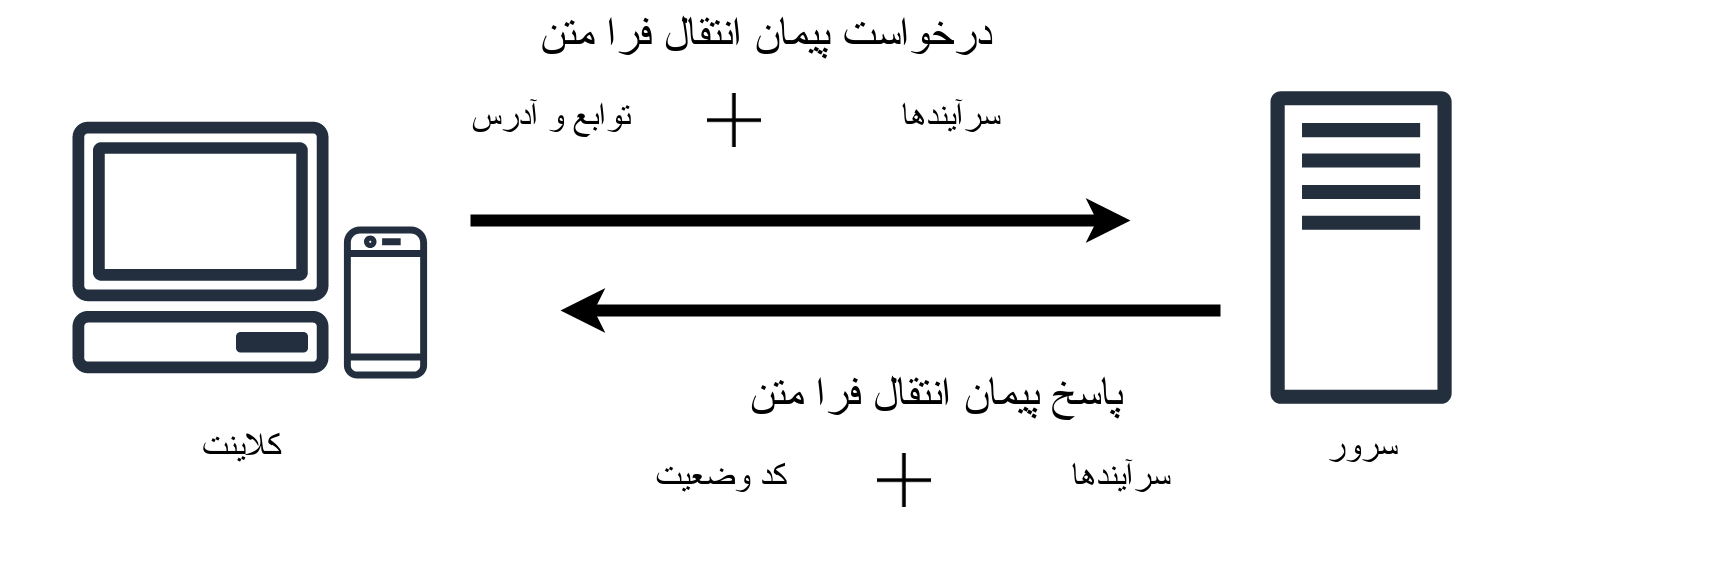
\includegraphics[width=\textwidth]{figs/http.png}}
        \caption{نمای کلی درخواست و پاسخ پیمان انتقال فرا متن}
        \label{fig:http}
    \end{figure}
}

\subsection{توابع پیمان انتقال فرا متن}
\label{subsec:http_methods}
\paragraph{}
{
    پیمان انتقال فرا متن توابع\footnote{\lr{پیمان انتقال فرا متن Methods}} مختلفی را برای تعیین نوع عملیاتی که باید انجام شود تعریف کرده است که عبارت است از:
    \begin{enumerate}
        \item دریافت\footnote{\lr{GET}}: این تابع برای دریافت (خواندن) اطلاعات از یک منبع مشخص درخواست می‌شود. مثلاً با استفاده از تابع دریافت می‌توانید صفحات وب، تصاویر یا سایر منابع را از سرور دریافت کنید. درخواست دریافت، بدون تغییر و اثری روی منبع مورد درخواست، انجام می‌شود.
        \item ساخت\footnote{\lr{POST}}: این تابع برای ارسال داده‌ها به سرور استفاده می‌شود. از تابع ساخت برای ایجاد یا ارسال داده جدید به سرور استفاده می‌شود، مانند ارسال فرم‌ها در وب، ارسال نظرات یا انجام عملیات‌های پردازشی. درخواست ساخت می‌تواند تغییراتی روی منبع مورد درخواست ایجاد کند.
        \item بروزرسانی\footnote{\lr{PUT}}: این تابع برای به‌روزرسانی (بازنویسی) یک منبع مشخص استفاده می‌شود. با استفاده از تابع بروزرسانی، می‌توانید اطلاعات موجود در سرور را با داده‌های جدید جایگزین کنید. درخواست بروزرسانی می‌تواند تغییراتی روی منبع مورد درخواست اعمال کند یا در صورت عدم وجود، یک منبع جدید ایجاد کند.
        \item حذف\footnote{\lr{DELETE}}: این تابع برای حذف یک منبع مشخص استفاده می‌شود. با استفاده از تابع حذف می‌توانید یک منبع را از سرور حذف کنید. درخواست حذف، منبع مورد نظر را از سرور حذف می‌کند.
        \item بروزرسانی مقطعی\footnote{\lr{PATCH}}: این تابع برای اعمال تغییرات جزئی روی یک منبع مشخص استفاده می‌شود. با استفاده از تابع بروزرسانی مقطعی، می‌توانید تغییرات کوچکی را روی یک منبع اعمال کنید بدون ایجاد تغییرات بزرگتری در داده‌های موجود.
    \end{enumerate}
    این توابع به عنوان پایه‌های پیمان انتقال فرا متن عمل می‌کنند و به کلاینت و سرور امکان ارتباط و انجام عملیات‌های مختلف را می‌دهند. درخواست‌ها و پاسخ‌های پیمان انتقال فرا متن بر اساس این توابع تعریف می‌شوند و برای تعامل موثر بین سرویس‌دهنده و کلاینت استفاده می‌شوند.
}

\subsection{درخواست پیمان انتقال فرا متن}
\label{subsec:http_requests}
\paragraph{}
{
    در پیمان انتقال فرا متن، وقتی که کلاینت (مانند مرورگر وب یا برنامه‌ای که درخواست ارسال می‌کند) برای دستیابی به منبع مورد نظر خود، درخواستی ایجاد می‌کند، یک درخواست پیمان انتقال فرا متن ایجاد می‌شود. درخواست‌های پیمان انتقال فرا متن شامل اطلاعاتی درباره نوع و منبع درخواست شده هستند. در زیر توضیحی از مهمترین اجزای یک درخواست پیمان انتقال فرا متن را می‌یابید:
    \begin{enumerate}
        \item توابع پیمان انتقال فرا متن: تابع مشخص می‌کند کلاینت درخواست انجام چه عملیاتی را بر روی منبع مورد نظر دارد.
        \item درس\footnote{\lr{Uniform Resource Locator (URL)}}: مشخص می‌کند که منبع مورد نظر کجا قرار دارد و آدرس دقیق آن چیست. آدرس شامل پروتکل، نام دامنه سرور\footnote{\lr{Domain Name}} و مسیر\footnote{\lr{Path}} منبع مورد نظر است.
        \item سرآیندها: درخواست پیمان انتقال فرا متن می‌تواند شامل سرآیندها باشد که اطلاعات اضافی درباره درخواست و مشخصات کلاینت را ارائه می‌دهند. به عنوان مثال، سرآیندها می‌توانند شامل اطلاعات مربوط به نوع محتوا، زبان مورد نظر، تاریخ و غیره باشند.
        \item بدنه درخواست\footnote{\lr{Request Body}}: بدنه درخواست، در صورتی که درخواست ارسالی دارای داده‌های ارسالی است، این داده‌ها را در خود نگه می‌دارد. بدنه درخواست به صورت متنی یا در قالب داده‌های باینری می‌تواند باشد و معمولاً در درخواست‌هایی مانند ساخت و بروزرسانی استفاده می‌شود.
    \end{enumerate}
    هنگامی که کلاینت درخواست پیمان انتقال فرا متن را به سرور ارسال می‌کند، سرور با استفاده از اطلاعات درخواست، منبع مورد نظر را پیدا کرده و به مناسبت درخواست، پاسخ مناسب را به کلاینت ارسال می‌کند. درخواست‌های پیمان انتقال فرا متن بسته به نوع و عملیات مورد نظر، تعیین می‌کنند که چه عملیاتی باید در سمت سرور انجام شود و اطلاعات مربوطه را برگردانند.
}

\subsection{پاسخ‌ پیمان انتقال فرا متن}
\label{subsec:http_responses}
\paragraph{}
{
    هنگامی که یک درخواست از سوی کلاینت به سرور ارسال می‌شود، سرور با یک پاسخ\footnote{\lr{پیمان انتقال فرا متن Response}} مناسب به آن درخواست پاسخ می‌دهد. پاسخ‌های پیمان انتقال فرا متن حاوی اطلاعات مربوط به نتیجه درخواست و وضعیت آن است.
    \begin{enumerate}
        \item کد وضعیت\footnote{\lr{Status Code}}: هر پاسخ پیمان انتقال فرا متن دارای یک کد وضعیت است که نشان می‌دهد درخواست با موفقیت انجام شده است یا با مشکل مواجه شده است. برخی از کدهای وضعیت رایج عبارتند از:
        \begin{enumerate}
            \item کد ۲۰۰: درخواست با موفقیت انجام شده است و پاسخ داده مورد نظر در دسترس است.
            \item کد ۴۰۴: منبع مورد نظر پیدا نشد.
            \item کد ۵۰۰: مشکلی در سمت سرور رخ داده است که موجب عدم توانایی در ارسال پاسخ مورد نظر شده است.
        \end{enumerate}
        \item سرآیندها: پاسخ پیمان انتقال فرا متن شامل سرآیندها است که اطلاعات اضافی در مورد پاسخ و منبع مورد نظر را ارائه می‌دهند. به عنوان مثال، سرآیندها می‌توانند شامل اطلاعات مربوط به نوع محتوا، طول پاسخ، تاریخ ارسال، و غیره باشند.
        \item محتوای پاسخ\footnote{\lr{Response Body}}: پاسخ پیمان انتقال فرا متن ممکن است حاوی محتوای مورد نظر باشد که توسط سرور ارسال می‌شود. محتوای پاسخ می‌تواند اطلاعاتی مانند متن، تصویر، ویدیو یا سایر منابع مورد نیاز را شامل شود.
    \end{enumerate}
    پاسخ‌های پیمان انتقال فرا متن ارسال شده توسط سرور معمولاً به درخواست‌های ارسالی از سوی مشتری پاسخ می‌دهند و اطلاعات مورد نیاز را در اختیار مشتری قرار می‌دهند. این پاسخ‌ها با کدهای وضعیت، سرآیندها و محتوای پاسخ کامل شده و تعیین می‌کنند که درخواست با موفقیت انجام شده است یا خطا رخ داده است.
}

\subsection{انتقال حالت نمایشی}
\label{subsec:rest}
\paragraph{}
{
    انتقال حالت نمایشی\footnote{\lr{Representational State Transfer (REST)}} یک معماری نرم‌افزاری است که برای طراحی سامنه‌های توزیع‌شده و مبتنی بر وب استفاده می‌شود. انتقال حالت نمایشی بر اساس مجموعه‌ای از اصول و محدودیت‌ها ساختاردهی شده است که در تبادل اطلاعات بین سرور و کلاینت نقش مهمی دارد. یکی از اصول اساسی انتقال حالت نمایشی، تعریف یکپارچگی\footnote{\lr{Uniform Interface}} برای سامنه است. این به این معنی است که سامنه باید یک مجموعه‌ی مشخص از روش‌های استاندارد را برای تعاملات در نظر بگیرد. معمولاً در سامنه‌های انتقال حالت نمایشی، از متدهای پیمان انتقال فرا متن مانند دریافت، ساخت، بروزرسانی و حذف برای تعیین عملیات مورد نیاز استفاده می‌شود. همچنین، منابع\footnote{\lr{Resources}} در سامنه انتقال حالت نمایشی به صورت یکتا شناسایی می‌شوند و آدرس‌های مشخصی برای آنها تعیین می‌شود.با توجه به این اصول و محدودیت‌ها، سامنه‌های انتقال حالت نمایشی قابلیت‌هایی مانند قابلیت توزیع، قابلیت مقیاس‌پذیری، انعطاف‌پذیری و قابلیت استفاده مجدد را فراهم می‌کنند. از طریق روش‌های استاندارد و اصول انتقال حالت نمایشی، سامنه‌ها قادر به تعامل با یکدیگر بدون توجه به جزئیات داخلی و پیچیدگی‌های نحوه پیاده‌سازی هستند.   
    \begin{figure}[H]
        \center{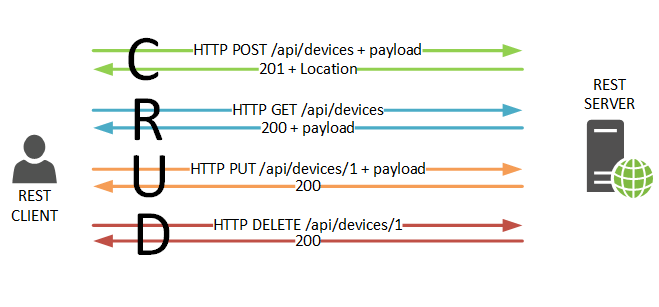
\includegraphics[width=\textwidth]{figs/rest-crud.png}}
        \caption{نمای کلی از انتقال حالت نمایشی}
        \label{fig:rest}
    \end{figure}
}

\subsection{رابط کاربردی قابل برنامه‌ریزی}
\label{subsecsec:api}
\paragraph{}
{
    رابط کاربردی قابل برنامه‌ریزی\footnote{\lr{Application Programming Interface}} به قوانین، پروتکل‌ها و دستوراتی گفته می‌شود که برای ارتباط و 
    تعامل بین نرم‌افزارها، خدمات و برنامه‌های مختلف به کار می‌رود. به طور کلی، رابط کاربردی قابل برنامه‌ریزی نقش یک میانجی بین سامانه‌ها را بازی
    می‌کند و به برنامه‌نویسان اجازه می‌دهد با استفاده از آن، به منابع و امکانات موجود در سامانه دیگر دسترسی پیدا کنند. رابط کاربردی قابل برنامه‌ریزی‌ها
    می‌توانند در دو شکل مختلف عمل کنند: به صورت وب خدمت یا به صورت کتابخانه برنامه‌نویسی. در حالت وب خدمت، رابط کاربردی قابل برنامه‌ریزی بر روی
    یک سرور میزبان شده است و از طریق پروتکل‌های اینترنتی مانند پیمان انتقال فرا متن قابل دسترسی است. در حالت کتابخانه برنامه‌نویسی، دستورات و توابع مشخصی به
    برنامه اضافه می‌شوند که برنامه‌نویسان می‌توانند از آنها به عنوان قسمتی از برنامه خود استفاده کنند. استفاده از رابط کاربردی قابل برنامه‌ریزی‌ها
    به برنامه‌نویسان امکان می‌دهد که بخشی از دستورات را استفاده کنند و از خدمات و قابلیت‌های ارائه شده توسط یک سامانه دیگر بهره ببرند. این 
    راهکار می‌تواند زمان و هزینه توسعه برنامه را کاهش داده و امکان ادغام بین نرم‌افزارها را فراهم کند. به طور خلاصه، رابط کاربردی قابل برنامه‌ریزی
    .مانند یک پل ارتباطی است که برنامه‌نویسان می‌توانند از آن استفاده کنند تا بین نرم‌افزارها و خدمات اطلاعات را به اشتراک بگذارند و تعامل کنند.
    \begin{figure}[H]
        \center{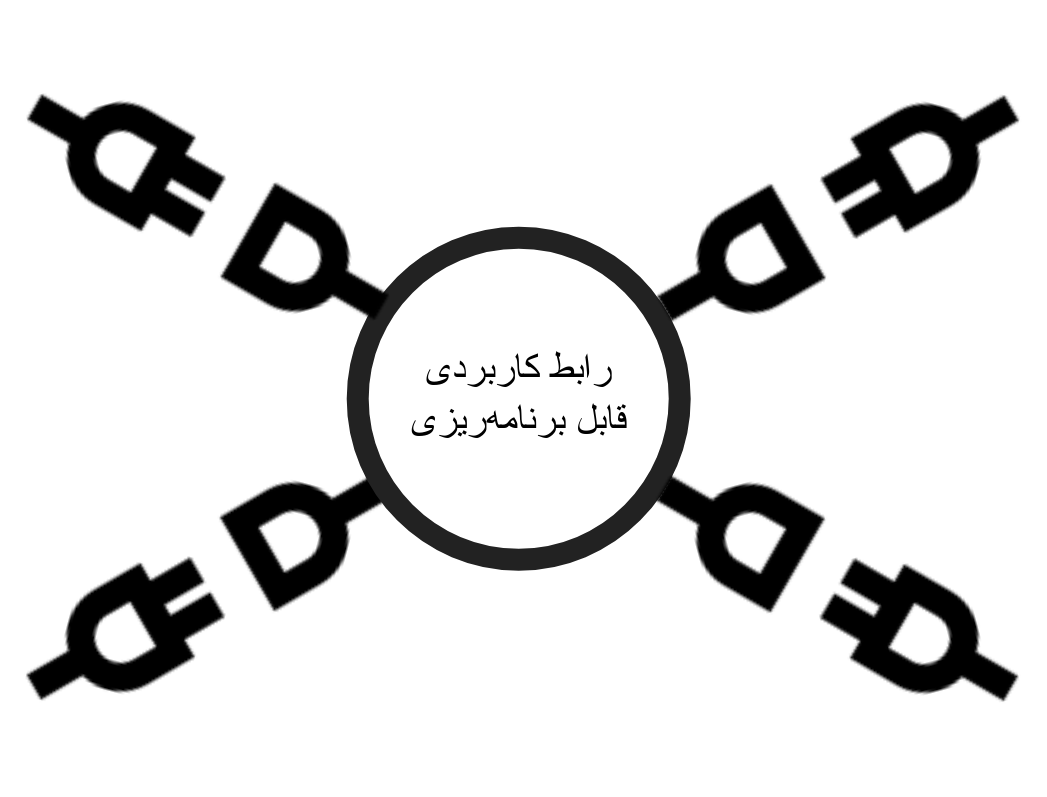
\includegraphics[width=\textwidth]{figs/api.png}}
        \caption{نمای کلی از رابط کاربردی قابل برنامه‌ریزی}
        \label{fig:api}
    \end{figure}
}

\section{معماری فن‌آوت}
\label{sec:fanout}
\paragraph{}
{
    معماری فن‌آوت\footnote{\lr{Fan-out}}: الگوی طراحی است که به طور معمول در سامانه‌های توزیع‌شده برای مدیریت همزمان یا موازی درخواست‌ها استفاده می‌شود. این معماری به توزیع درخواست‌های ورودی به چند واحد پردازش ، که به عنوان کارگرها شناخته می‌شوند، برای انجام عملیات مورد نیاز می‌پردازد. معماری فن‌آوت با بهره‌گیری از پردازش موازی و توازن بار، امکان مقیاس‌پذیری و بهبود عملکرد سیستم را فراهم می‌کند. در معماری فن‌آوت، هنگامی که یک درخواست دریافت می‌شود، آن را به چندین کارگر مستقل تکرار یا ارسال می‌کنند تا هر کدام از آن‌ها قادر به پردازش درخواست به صورت مستقل باشند. این رویکرد به چندین کارگر اجازه می‌دهد تا به صورت همزمان روی بخش‌های مختلف درخواست کار کنند و بهبود ظرفیت تولید و کاهش زمان پاسخ را به همراه داشته باشد.
}

\section{کوبلت مجازی}
\label{sec:vritkubelet}
\paragraph{}
{
    کوبلت مجازی\footnote{\lr{Virtual Kubelet}} یک پروژه متن باز است که با گسترش رابط‌ کاربردی قابل برنامه‌ریزی کوبرنیتز، امکان ادغام\footnote{\lr{Integration}} خدمات و سامانه‌های خارجی را در قالب گره‌های کوبرنیتز فراهم می‌کند. این پروژه این امکان را می‌دهد که یک گره "مجازی" بسازیم که توسط کوبرنیتز قابل مدیریت باشد و امکان ادغام سامانه‌های متنوع را در داخل خوشه کوبرنیتز به صورت یک‌پارچه فراهم کند.    
    \begin{figure}[H]
     \center{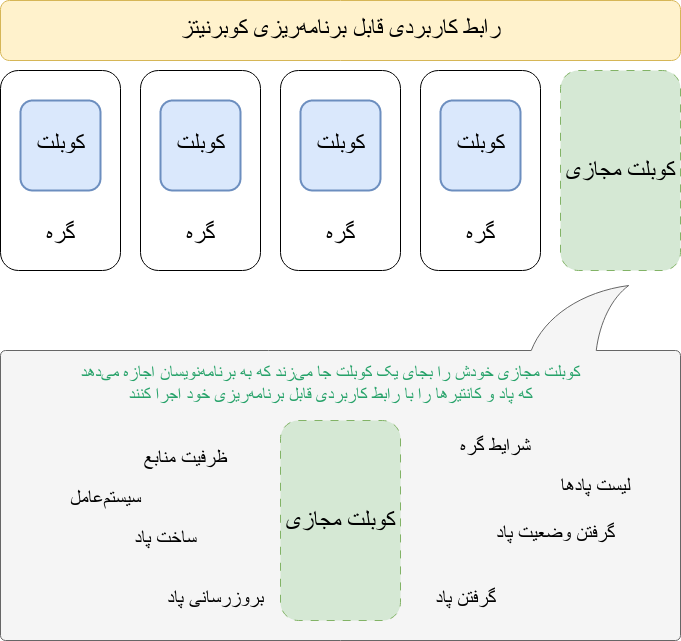
\includegraphics[width=0.8\textwidth]{figs/vkube.png}}
     \caption{کوبلت مجازی در یک خوشه کوبرنیتز}
     \label{fig:virtkublet_arch}
    \end{figure}
}

\subsection{معماری کوبلت مجازی}
\label{subsec:vkube_arch}
\paragraph{}
{
    کوبلت مجازی از چندین بخش کلیدی تشکیل شده است:
    \begin{enumerate}
        \item تامین‌کننده: تامین‌کننده مسئول پیاده‌سازی رابط کوبلت مجازی است و به عنوان پل ارتباطی بین سامانه یا خدمت خارجی و کوبرنیتز عمل می‌کند. این بخش، فراخوانی‌های رابط کاربردی قابل برنامه‌ریزی کوبرنیتز را به عملیات مناسب در سامانه خارجی ترجمه می‌کند.
        \item گره: گره مجازی نمایانگر یک سامانه یا خدمت خارجی در خوشه کوبرنیتز است. عملکرد آن شبیه یک گره کوبرنیتز عادی است، اما به جای اجرا در زیرساخت فیزیکی، از طریق تامین‌کننده با سامانه خارجی ارتباط برقرار می‌کند.
        \item پاد: پاد در کوبرنیتز، شامل یک یا چند کانتینر است. در کوبلت مجازی، پادها نماینده کارها\footnote{\lr{Workload}} هستند که در گره‌های مجازی ایجاد شده توسط سامانه خارجی اجرا می‌شوند.
        \item برنامه‌ریز\footnote{\lr{Scheduler}}: برنامه‌ریز کوبرنیتز مسئول تخصیص پادها به گره‌های موجود بر اساس نیازهای منابع و محدودیت‌ها است. در کوبلت مجازی، برنامه‌ریز مسئول زمانبندی پادها به گره‌های مجازی ایجاد شده توسط تامین‌کننده است. این بخش تضمین می‌کند که منابع بصورت بهینه استفاده شده و کارها به طور مناسب در سامانه خارجی توزیع شوند.
    \end{enumerate}
}

\section{اینترنت اشیاء}
\label{sec:iot}
\paragraph{}
{   
    اینترنت اشیاء\footnote{\lr{Internt of Things (IoT)}} به مجموعه‌ای از دستگاه‌ها، سنسورها، دستگاه‌های هوشمند و شبکه‌های مرتبط که قادر
    به تبادل اطلاعات با یکدیگر از طریق اتصال به اینترنت هستند، اشاره دارد. این اشیاء می‌توانند شامل تلفن همراه‌ها و ساعت هوشمند تا لوازم
    خانگی هوشمند، خودروهای متصل و تجهیزات صنعتی باشند. اینترنت اشیاء با اتصال اشیاء و جمع‌آوری اطلاعات، امکان برقراری ارتباط و کنترل 
    بیشتری را بین دنیای فیزیکی و دنیای دیجیتال فراهم می‌کند. مزیت اصلی اینرنت اشیاء در جمع‌آوری و تبادل داده‌ها است. سنسورها و دستگاه‌ها 
    در اینترنت اشیاء می‌توانند اطلاعات مربوط به بستر، شرایط، موقعیت جغرافیایی، وضعیت و داده‌های دیگر را جمع‌آوری کرده و به سرورها یا سامانه‌های 
    مرکزی ارسال کنند. این اطلاعات در سرورها تحلیل می‌شوند و می‌توانند به عنوان منبعی برای ارائه داده‌های مفید، تجزیه و تحلیل ترافیک، پیش‌بینی و 
    اتخاذ تصمیم‌های هوشمند استفاده شوند. از جمله کاربردهای اینترنت اشیاء می‌توان به موارد زیر اشاره کرد:
    \begin{enumerate}
        \item خانه هوشمند: اتصال لوازم خانگی مانند تلویزیون، سامانه‌های روشنایی، دستگاه‌های گرمایشی و سرمایشی، سامانه‌های امنیتی و سایر دستگاه‌ها به اینترنت به کاربران امکان می‌دهد تا این دستگاه‌ها را از راه دور کنترل و مدیریت کنند.
        \item صنعت هوشمند: در صنعت، اینترنت اشیاء می‌تواند در جمع‌آوری داده‌ها از تجهیزات و سنسورها به منظور نظارت بر فرآیندها، پیشگیری از خرابی‌ها، بهینه‌سازی استفاده از منابع و افزایش بهره‌وری مورد استفاده قرار گیرد.
        \item شهر هوشمند: با استفاده از سنسورها و دستگاه‌های اینترنت اشیاء، می‌توان شهرها را هوشمندتر کرده و بهبود امکانات شهری مانند مدیریت ترافیک، پارکینگ هوشمند، مدیریت پسماند و رصد آلودگی هوا را فراهم کرد.
        \item سلامتی هوشمند: استفاده از دستگاه‌های پوشیدنی، سنسورها و دستگاه‌های پزشکی هوشمند، امکان نظارت بر سلامتی فرد، جمع‌آوری داده‌های پزشکی، پیشگیری از بیماری‌ها و ارائه مراقبت بهتر را فراهم می‌کند.
    \end{enumerate}
    به طور کلی، اینترنت اشیاء با اتصال اشیاء به اینترنت و جمع‌آوری داده‌ها، امکانات جدیدی را در دسترس قرار می‌دهد و قابلیت های جدیدی را برای کنترل، مدیریت و بهبود عملکرد اشیا فراهم می‌کند.
    \begin{figure}[H]
        \center{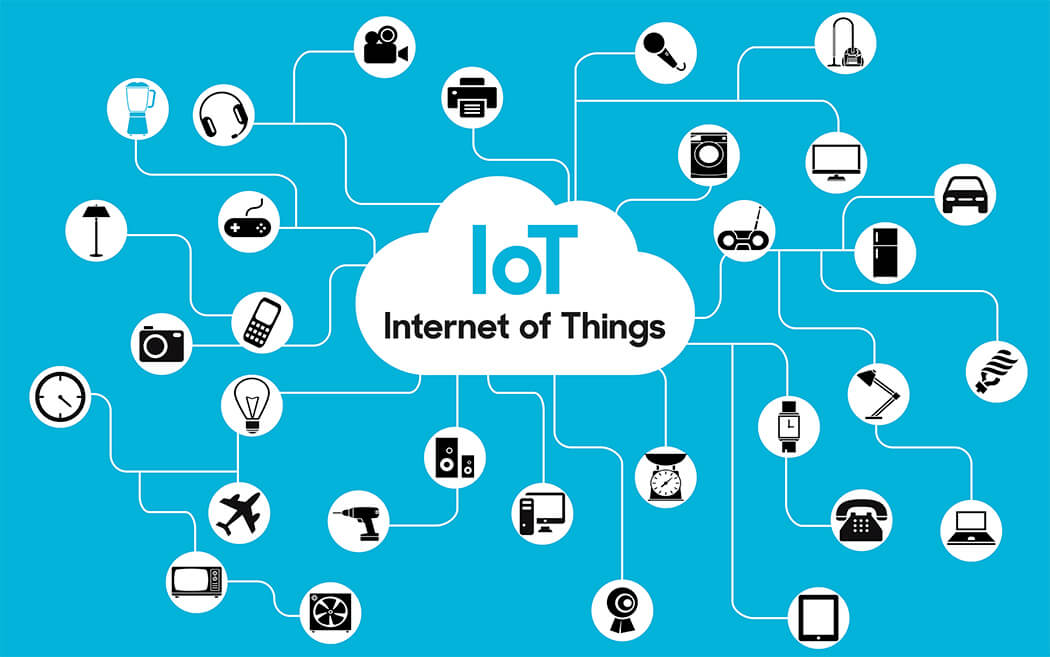
\includegraphics[width=0.9\textwidth]{figs/iot.jpg}}
        \caption{نمای کلی از اینترنت اشیاء}
        \label{fig:iot}
    \end{figure}
}

% \section{شبکه‌های عصبی بازگشتی}
% \label{sec:rnn}
% \paragraph{}
% {
%     باید توجه داشت که استفاده از شبکه‌های عصبی مصنوعی برای داده‌های دنباله‌ای عملی
%     نیست. به عبارتی دیگر در شبکه‌های عصبی مصنوعی فرض می‌کنیم که داده‌های ورودی به صورت
%     کامل مستقل از یکدیگرند. با توجه به این فرضیه شبکه‌های عصبی مصنوعی عادی برای 
%     استخراج وابستگی بین دنباله‌ها 
%     (برای مثال کلمات درون یک جمله)
%     کارآمد نیستند. برای در نظر گرفتن این وابستگی، از شبکه‌های عصبی بازگشتی استفاده
%     می‌شود. 

%     شبکه‌های عصبی بازگشتی را می‌توان همان شبکه‌های عصبی عادی با یک حافظه در نظر گرفت.
%     در واقع مهم‌ترین تفاوت شبکه‌های عصبی بازگشتی وجود حالت‌های مخفی است که می‌توانند 
%     اطلاعات گذشته را در حافظه نگه دارند و سپس از طریق پس‌انتشار خطا در راستای زمان 
%     به کاهش تابع هزینه کمک کنند. قابلیت به یاد سپردن گذشته شبکه‌های عصبی بازگشتی را
%     بسیار کارآمد کرده است. در واقع شبکه‌های عصبی بازگشتی با تعداد پارامترهای محدود
%     تورینگ‌‌کامل هستند و توانایی پیاده‌سازی هر الگوریتمی را دارند. 
%     \cite{sontag1995computational}

%     \begin{figure}[H]
%      \center{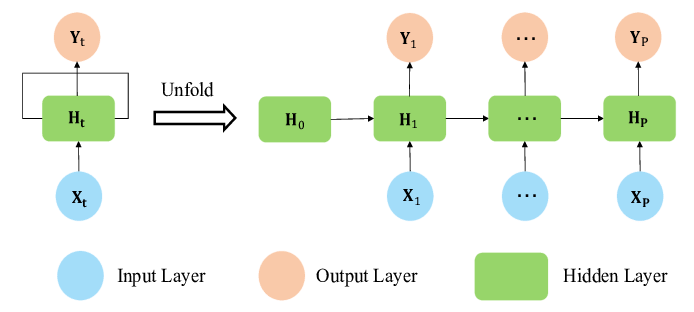
\includegraphics[width=0.7\textwidth]{figs/RNN_ARC_1.png}}
%      \caption{معماری کلی شبکه‌های عصبی بازگشتی}
%      \label{fig:rnn_1}
%     \end{figure}

%     یکی از مشکلات متداول شبکه‌های عصبی بازگشتی، محو شدگی و انفجار گرادیان
%     به صورت نمایی در گذر زمان است. این مسئله بدان معنی است که این معماری‌ها 
%     توانایی پردازش دنباله‌هایی با وابستگی‌های طولانی را ندارند. برای حل این‌ مشکل
%     معماری‌های متفاوتی ارائه شد که به بررسی مهم‌ترین آن‌ها می‌پردازیم. 
% }

% \subsection{
%     حافظه طولانی کوتا‌ه‌مدت
% }
% \label{subsec:lstm}
%  {
%     در سال 1977 یک معماری از شبگه‌های عصبی بازگشتی به نام  حافظه طولانی کوتا‌ه‌مدت 
%     ارائه شد. هر عنصر از شبکه شامل یک درگاه ورودی، یک سلول، یک درگاه
%     فراموشی و یک درگاه خروجی است. سلول طولانی کوتا‌ه‌مدت وظیفه یادآوری 
%     مقادیر دیده‌شده در گذشته را برعهده دارد، در حالی که درگاه‌های ورودی، 
%     فراموشی و خروجی وظیفه کنترل جریان داده‌ها را دارند. 

%     \begin{figure}[H]
%         \center{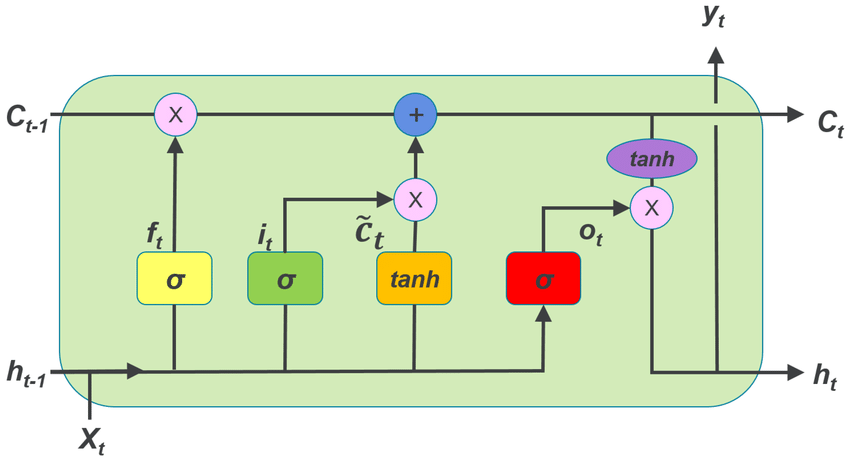
\includegraphics[width=0.7\textwidth]{figs/LSTM_ARC_1.png}}
%         \caption{معماری حافظه کوتاه‌مدت طولانی‌مدت}
%         \label{fig:lstm_1}
%     \end{figure}
   
%     از آنجایی که هدف اصلی حل محوشدگی نمایی گرادیان در طول زمان بود، حافظه‌های 
%     طولانی کوتا‌ه‌مدت قابلیت پردازش دنباله‌های طولانی‌‌تری را دارند. معادلات مرتبط با
%     این شبکه‌ها در زیر آورده شده است.

%     \begin{center}
%         \begin{equation} \label{eq:2}
%             \sigma (x) = \frac{1}{1 + e ^{-x}}
%         \end{equation}
%         \begin{equation} \label{eq:3}
%             tanh(x) = \frac{e^{2x} - 1}{e^{2x} + 1}
%         \end{equation}
%         \begin{equation} \label{eq:4}
%             i_t = \sigma (W_i^T x_t + W_i^T h_{t - 1} + b_i)
%         \end{equation}
%         \begin{equation} \label{eq:5}
%             f_t = \sigma (W_f^T x_t + W_f^T h_{t - 1} + b_f)
%         \end{equation}
%         \begin{equation} \label{eq:6}
%             o_t = \sigma (W_o^T x_t + W_o^T h_{t - 1} + b_o)
%         \end{equation}
%         \begin{equation} \label{eq:7}
%             c_t = f_t \circ c_{t - 1} +
%                 i_t \circ tanh(W_c x_t + U_c h_{t - 1} + b_c)
%         \end{equation}
%         \begin{equation} \label{eq:8}
%             h_t = o_t \circ tanh(c_t)
%         \end{equation}
%     \end{center}

%     سلول 
%     (معادله \ref{eq:8})
%     وابستگی‌های بین مقادیر ورودی در دنباله را نگه می‌دارد. درگاه ورودی
%     (معادله \ref{eq:4})
%     وظیفه انتخاب ویژگی‌های ورودی برای عبور به سلول را عهده‌دار است. 
%     درگاه فراموشی 
%     (معادله \ref{eq:5})
%     میزان این که یک مقدار چقدر در سلول باقی بماند را برعهده دارد و در نهایت 
%     درگاه خروجی، میزان مشارکت مقادیر موجود در سلول را برای محاسبه خروجی را 
%     کنترل می‌کند. 
% }

% \subsection{
%     واحد بازگشتی دروازه‌دار    
% }
% \label{subsec:rep_learn}
% \paragraph{}
% {
%    در سال 2014 شبکه‌های واحد بازگشتی دروازه‌دار به عنوان معماری متفاوتی برای
%    شبکه‌های عصبی بازگشتی ارائه شد تا مشکل محوشدگی گرادیان‌ در حال آموزش را حل کند.
%    این واحد شباهت زیادی به حافظه طولانی کوتاه‌مدت دارد ولی در عین‌ حال تعداد
%    پارامترهای کمتری دارد و در نتیجه سریع‌تر آموزش می‌بیند. 

%    \begin{center}
%         \begin{equation} \label{eq:9}
%             z_t = \sigma (W_z x_t + U_z h_{t - 1} + b_z)
%         \end{equation}
%         \begin{equation} \label{eq:10}
%             r_t = \sigma (W_r x_t + U_r h_{t - 1} + b_r)
%         \end{equation}
%         \begin{equation} \label{eq:11}
%             \hat{h_t} = tanh (W_h x_t + U_r (r_t \circ h_{t - 1}) + b_h)
%         \end{equation}
%         \begin{equation} \label{eq:12}
%             h_t = (1 - z_t) \circ h_{t - 1} + z_t \circ \hat{h_t}
%         \end{equation}
%     \end{center}
    
%     مطابق با معادله 
%     \ref{eq:9}
%     درگاه $z_t$
%     مسئولیت تعیین عبور مقادیر برای استفاده در آینده را دارد. به عبارتی اگر 
%     مقدار آن برابر 1 باشد، بدان معنی است که شبکه مقدار بردار 
%     $h_t$ 
%     را به صورت کامل به‌روز و اطلاعات گذشته را فراموش می‌کند. متقابلا اگر 
%     مقدار این درگاه به 0 نزدیک باشد، شبکه مقادیر $h_t$ 
%     را از گذشته انتخاب می‌کند. درگاه فراموشی، مطابق با معادله
%     \ref{eq:10}
%     مسئولیت تعیین تاثیرگذاری مقادیر حالت قبلی در محاسبه حالت فعلی را بر عهده‌دارد.

%     \begin{figure}[H]
%         \center{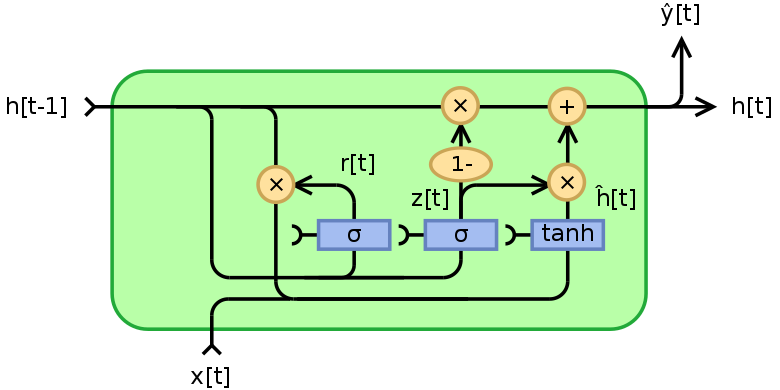
\includegraphics[width=0.7\textwidth]{figs/GRU_ARC_1.png}}
%         \caption{معماری شبکه واحد بازگشتی دروازه‌دار}
%         \label{fig:gru_1}
%     \end{figure}
% }
% \section{مدل‌های دنباله‌به‌دنباله}
% \label{sec:seq2seq}
% \paragraph{}{
%     مدل‌های دنباله‌به‌دنباله وظیفه تبدیل دنباله‌ها از یک دامنه به دنباله‌ای دیگر 
%     را برعهده دارند. به طور کلی این مدل‌ها دنباله‌ای با طول متغیر را ورودی می‌گیرند و
%     دنباله‌ای دیگر با طول متغیر بدل می‌کنند کع لزما طول آن با ورودی یکسان نیست. 
%     مدل‌های دنباله‌به‌دنباله دارای دو شبکه مجزا هستند. یک شبکه به عنوان کدگذار
%     که وظیفه تبدیل ورودی‌ها به یک یا چند بردار ویژگی را برعهده دارد. 
%     این بردار ویژگی یک بازنمایی از دنباله ورودی است که حداکثر معانی قابل
%     استخراج از دنباله ورودی را در بر دارد. شبکه دیگری با عنوان کدگشا 
%     برای تولید دنباله هدف آموزش می‌بیند. ورودی این بخش همان بردار ویژگی 
%     بدست آمده از کدگذار است. معمولا شبکه‌های کدگذار و کدگشا با یکدیگر آموزش
%     داده می‌شوند که به معنی پس انتشار خطا از کدگشا به کدگذار است. در شکل
%     \ref{fig:enc_dec_1}
%     نمونه‌ای از مدل‌های دنباله‌به‌دنباله را برای حل ترجمه ماشینی مشاهده می‌شود. 
%     \begin{figure}[H]
%         \center{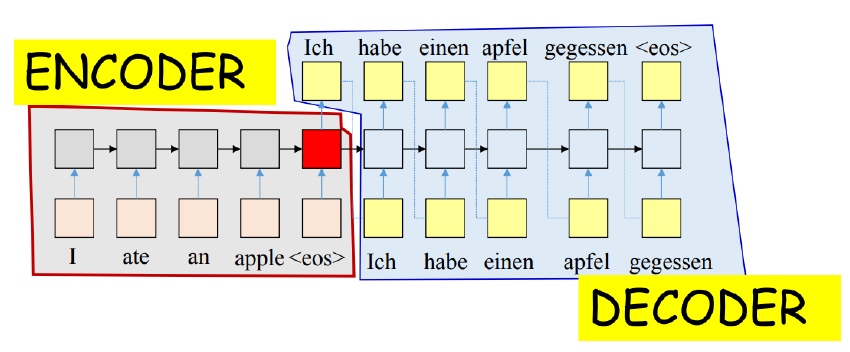
\includegraphics[width=0.7\textwidth]{figs/enc_dec.png}}
%         \caption{نمونه‌ای از معماری‌ کدگذار-کدگشا برای حل مسئله ترجمه ماشینی}
%         \label{fig:enc_dec_1}
%     \end{figure}
% }
% \section{مکانیزم توجه}
% \label{sec:attn}
% \paragraph{}{
%     شبکه‌های عصبی بازگشتی و معماری‌های مشابه آن می‌توانند اطلاعات درون یک 
%     دنباله را پردازش کنند و بر اساس آن‌ها نتیجه گیری کنند. حال فرض کنیم
%     که یک پاراگراف طولانی داریم و پس از خواندن آن سوالی پرسیده شود.
%     پس از روبه‌رو شدن با سوال، ممکن است متن را به صورت کامل به یاد نیاوریم
%     و لازم باشد که دوباره با توجه بیشتری به برخی جملات متن را بخوانیم.
%     بنابراین، توجه را می‌توانیم رفتار تمرکز بر روی بخش گسسته‌ای از اطلاعات 
%     و در نظر نگرفتن دیگر اجزاء تعریف کنیم. در ادامه به ایده‌ها و انواع 
%     مکانیزم‌های توجه ارائه شده در طی سال‌های گذشته می‌پردازیم.
% }
% \subsection{
%     مکانیزم توجه باهدانا 
%     (\lr{Bahdanau})
% }
% \label{subsec:bahdanau_attn}
% \paragraph{}{
%     در سال 2014 مکانیزمی 
%     \cite{DBLP:journals/corr/BahdanauCB14}
%     برای توجه به حالت‌های مخفی در محاسبه خروجی ارائه داد. در این معماری 
%     علاوه بر حالت سلول کدگذار آخر، تمام خروجی‌های کدگذار را به کدگشا می‌فرستیم
%     تا در هر گام، کدگشا یک جمع وزن‌دار بین خروجی‌ها حساب کند. وزن‌های این جمع، 
%     مفهوم توجه را پیاده‌سازی می‌کنند. هر حالتی که وزن بیشتری داشته‌باشد توجه
%     بیشتری را جلب می‌کند‍!
%     \begin{figure}[H]
%         \center{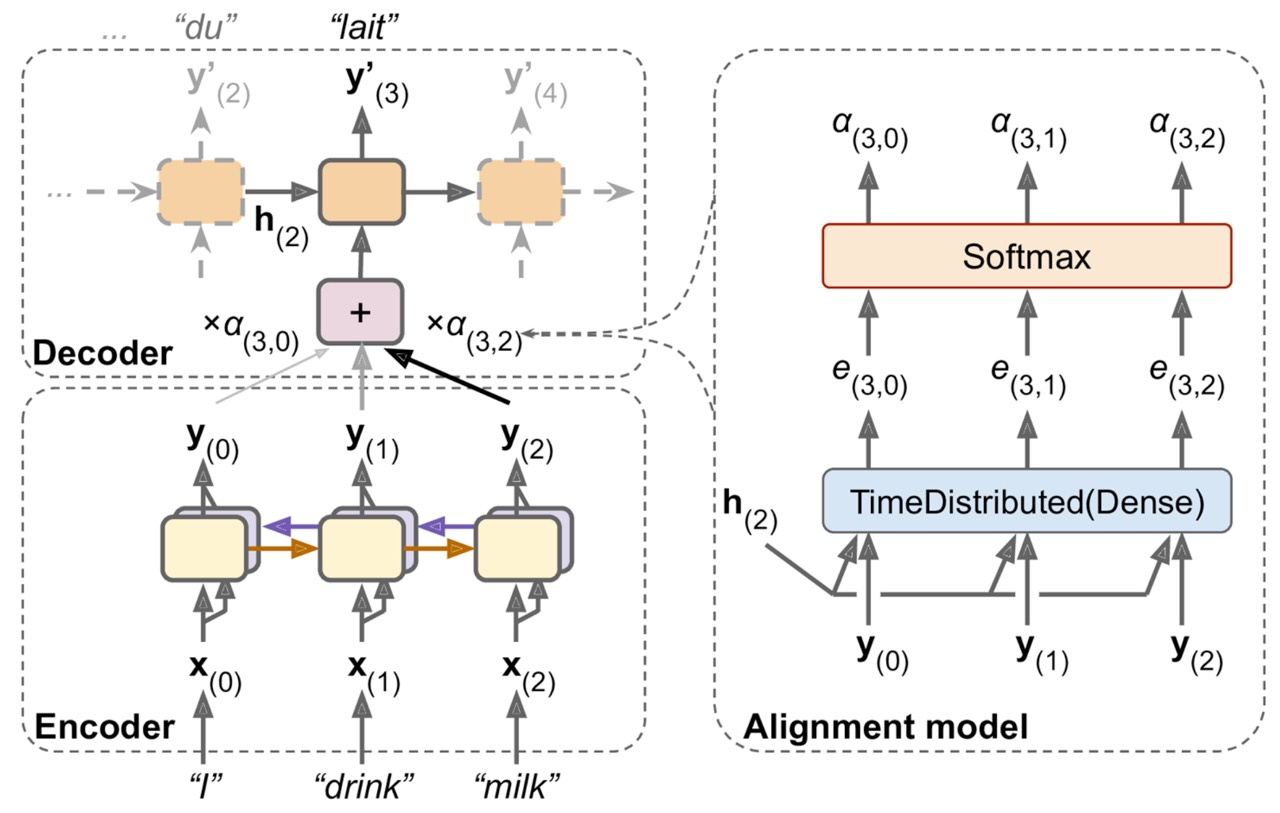
\includegraphics[width=0.7\textwidth]{figs/bahdanau_attn_1.jpeg}}
%         \caption{مکانیزم توجه باهدانا در ترجمه ماشینی}
%         \label{fig:bahdanau_attn}
%     \end{figure}

%     وزن‌های مذکور همان 
%     $\alpha$
%     موجود در شکل
%     \ref{fig:bahdanau_attn}
%     که همراه با شبکه آموزش می‌بینند. با توجه به شکل متوجه می‌شویم به هنگام
%     ترجمه کلمه 
%     \lr{lait}
%     ،
%     توجه بیشتری به کلمه متناظر آن که 
%     \lr{milk}
%     است، می‌شود. در ادامه به بررسی فرمول‌های مکانیزم توجه باهدانا می‌پردازیم. 

%     \begin{center}
%         \begin{equation} \label{eq:13}
%             e_{t, i} = a(s_{t - 1}, h_i)
%         \end{equation}
%         \begin{equation} \label{eq:14}
%             a(s_{t - 1}, h_i) = v^T tanh( W[{h_i; s_{t - 1}}] )
%         \end{equation}
%         \begin{equation} \label{eq:15}
%             a(s_{t - 1}, h_i) = v^T tanh( W[{W_1 h_i + W_2 s_{t - 1}}] )
%         \end{equation}
%         \begin{equation} \label{eq:16}
%             \alpha_{t, i} = softmax(e_{t, i})
%         \end{equation}
%     \end{center}

%     با توجه به معادله 
%     \ref{eq:16}،
%     برای محاسبه مقادیر 
%     $\alpha$
%     لازم است از تابع تناظر 
%     $a$ 
%     استفاده کنیم که برای محاسبه آن نیز دو روش الحاق 
%     (معادله \ref{eq:14})
%     و جمع 
%     (معادله \ref{eq:15})
%     وجود دارد. 
%     در نهایت با استفاده از یک لایه 
%     softmax
%     به محاسبه وزن‌ها می‌پردازیم. 
% }

% \subsection{
%     مکانیزم توجه لوآنگ 
%     (\lr{Luong})
% }
% \label{subsec:loung}
% \paragraph{}{
%     در سال 2015،
%     مقاله‌ای دیگر 
%     \cite{luong-etal-2015-effective}
%     مدل مکانیزم دیگری ارائه داد. از آنجایی که هدف مکانیزم توجه، 
%     محاسبه شباهت‌های بین خروجی‌های کدگذار و حالت‌های پنهان مراحل قبل کدگشا است،
%     در این مقاله نیز از ضرب کسینوسی استفاده شده است. همانطوری که از معادلات
%     زیر مشخص است، توجه لوآنگ، بر خلاف توجه باهدانا، از حالت پنهان 
%     $s_t$
%     استفاده می‌کند. 

%     \begin{center}
%         \begin{equation} \label{eq:17}
%             a(s_{t}, h_i) = v_a^T tanh( W[{h_i; s_{t}}] )
%         \end{equation}
%         \begin{equation} \label{eq:18}
%             a(s_{t}, h_i) = s_t^T h_i
%         \end{equation}
%         \begin{equation} \label{eq:19}
%             a(s_{t}, h_i) = s_t^T W_a h_i
%         \end{equation}
%     \end{center}
% }

% \subsection{
%     مکانیزم توجه به خود
% }
% \label{subsec:self_attn}
% \paragraph{}{
%     این مفهوم برای اولین بار در سال 2016 مطرح شد.
%     \cite{cheng-etal-2016-long}
%     هدف این توجه
%     این‌است که ارتباط اجزای موجود در یک دنباله را با یکدیگر بسنجد
%     تا بتواند برداشت درست‌تری از کل دنباله داشته باشد. تنها تفاوت 
%     این مکانیزم با توجه عادی این است میزان توجه اجزا دنباله را با خود
%     همان دنباله می‌سنجیم. شکل
%     \ref{fig:self_attention}
%     ارتباط کلمه‌ قرمز رنگ با کلمه‌های قبلی در جمله بررسی شده و شدت آبی بودن
%     هر کلمه، میزان ارتباط را نشان می‌دهد. 
%     \begin{figure}[H]
%         \center{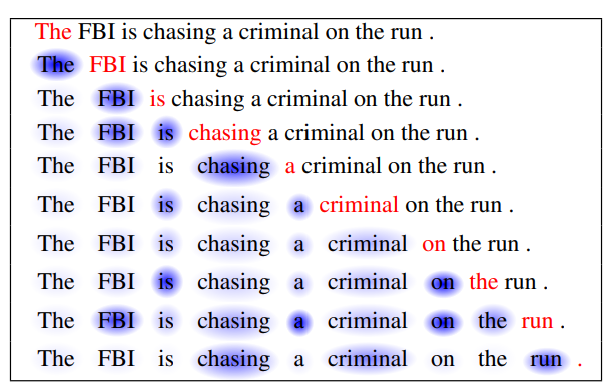
\includegraphics[width=0.7\textwidth]{figs/self_attn_1.png}}
%         \caption{نمونه‌ای از توجه به خود در یک جمله}
%         \label{fig:self_attn_1}
%     \end{figure}
% }


% \section{
%     مدل‌های transformer و مکانیزم توجه آن‌ها
% }
% \label{sec:transformers}
% \paragraph{}{
%     مدل‌های تبدیل‌کننده روش جدیدی را برای استفاده‌ از مفهوم توجه ارائه دادند.
%     در مقاله‌‌ی «توجه و دیگر هیچ!» 
%     \cite{NIPS2017_3f5ee243}
%     که در سال 2017 ارائه شد، این مدل‌ها مطلقا بر پایه 
%     مکانیزم توجه به خود تکیه کرده‌اند. اکثر این مدل‌ها به صورت 
%     مدل‌های دنباله‌به‌دنباله پیاده‌سازی شده‌اند به صورتی که دو بخش
%     کدگذار و کدگشا دارند. مطابق با شکل
%     \ref{fig:transformers_arc_1}
%     مشاهده‌ می‌کنیم که بخشی به نام  
%     \lr{Positional Embedding}
%     شرایط پردازش کلمات با توجه به جایگاه آن‌ها در جمله را فراهم می‌کند. 
%     برای این کار از معادلات 
%     \ref{eq:20} و \ref{eq:21}
%     بردارهای جایگاه محاسبه می‌شوند و به بردار‌های 
%     \lr{embedding}
%     اضافه می‌شوند. 
%     \begin{center}
%         \begin{equation} \label{eq:20}
%             PE(pos, 2i) = sin(\frac{pos}{10000^{\frac{2i}{d}}})
%         \end{equation}
%         \begin{equation} \label{eq:21}
%             PE(pos, 2i + 1) = cos(\frac{pos}{10000^{\frac{2i}{d}}})
%         \end{equation}
%     \end{center}
%     \begin{figure}[H]
%         \center{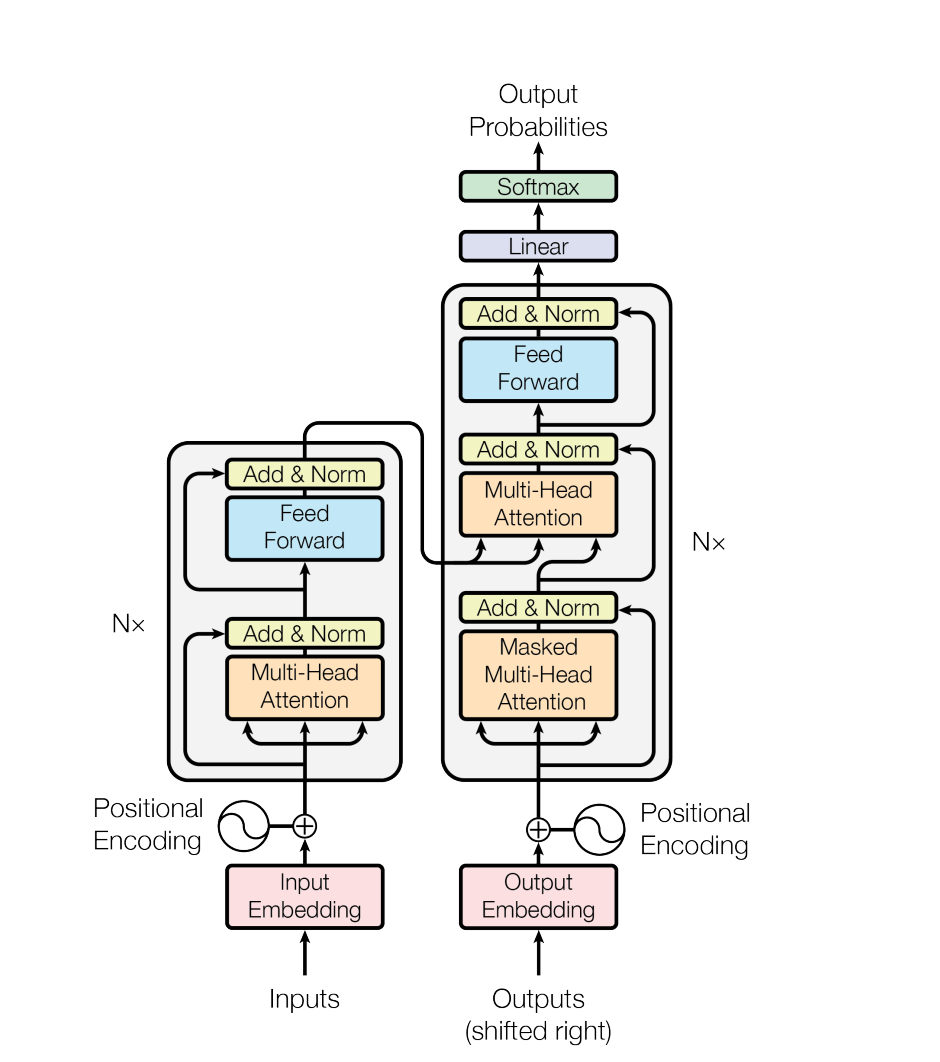
\includegraphics[width=0.7\textwidth]{figs/transformers_arc_1.png}}
%         \caption{مدل‌ تبدیل‌شونده و معماری آن‌}
%         \label{fig:transformers_arc_1}
%     \end{figure}

%     همان‌طوری که در شگل 
%     \ref{fig:transformers_arc_1} 
%     مشخص است، شبکه‌های کدگذار و کدگشا از توجه چندسر استفاده می‌کنند. 
%     این نوع از مکانیزم توجه را می‌توان تعمیم‌یافته‌ی نسخه قبلی آن دانست. 
%     در توجه چندسر ما با سه موجودیت مختلف به نام کلید 
%     (\lr{Key})، 
%     مقدار 
%     (\lr{Value})
%      و پرسش 
%     (\lr{Query})
%     سروکار داریم. 
%     در مبحث توجه گفتیم که هدف این کار، تعیین میزان ارتباط بین هر جزء جمله خروجی
%     با تمامی اعضای جمله ورودی است.
%     اگر به شکل 
%     \ref{fig:transformers_arc_1} 
%     توجه کنید، می‌بینید که هر سه ورودی این بلوک توجه 
%     از یک منبع که همان جمله‌ی ورودی است می‌آیند، پس از نوع توجه به خود  
%     است و هدف آن تعیین ارتباط و درک بهتر اجزای جمله‌ی زبان مبدا به یکدیگر است.
%     پیش از بررسی ادامه‌ی روند مدل، لازم است تا الگوریتمی
%     که در این نوع از مکانیزم توجه دنبال می‌شود را بررسی کنیم.
    
%     \begin{figure}[H]
%         \center{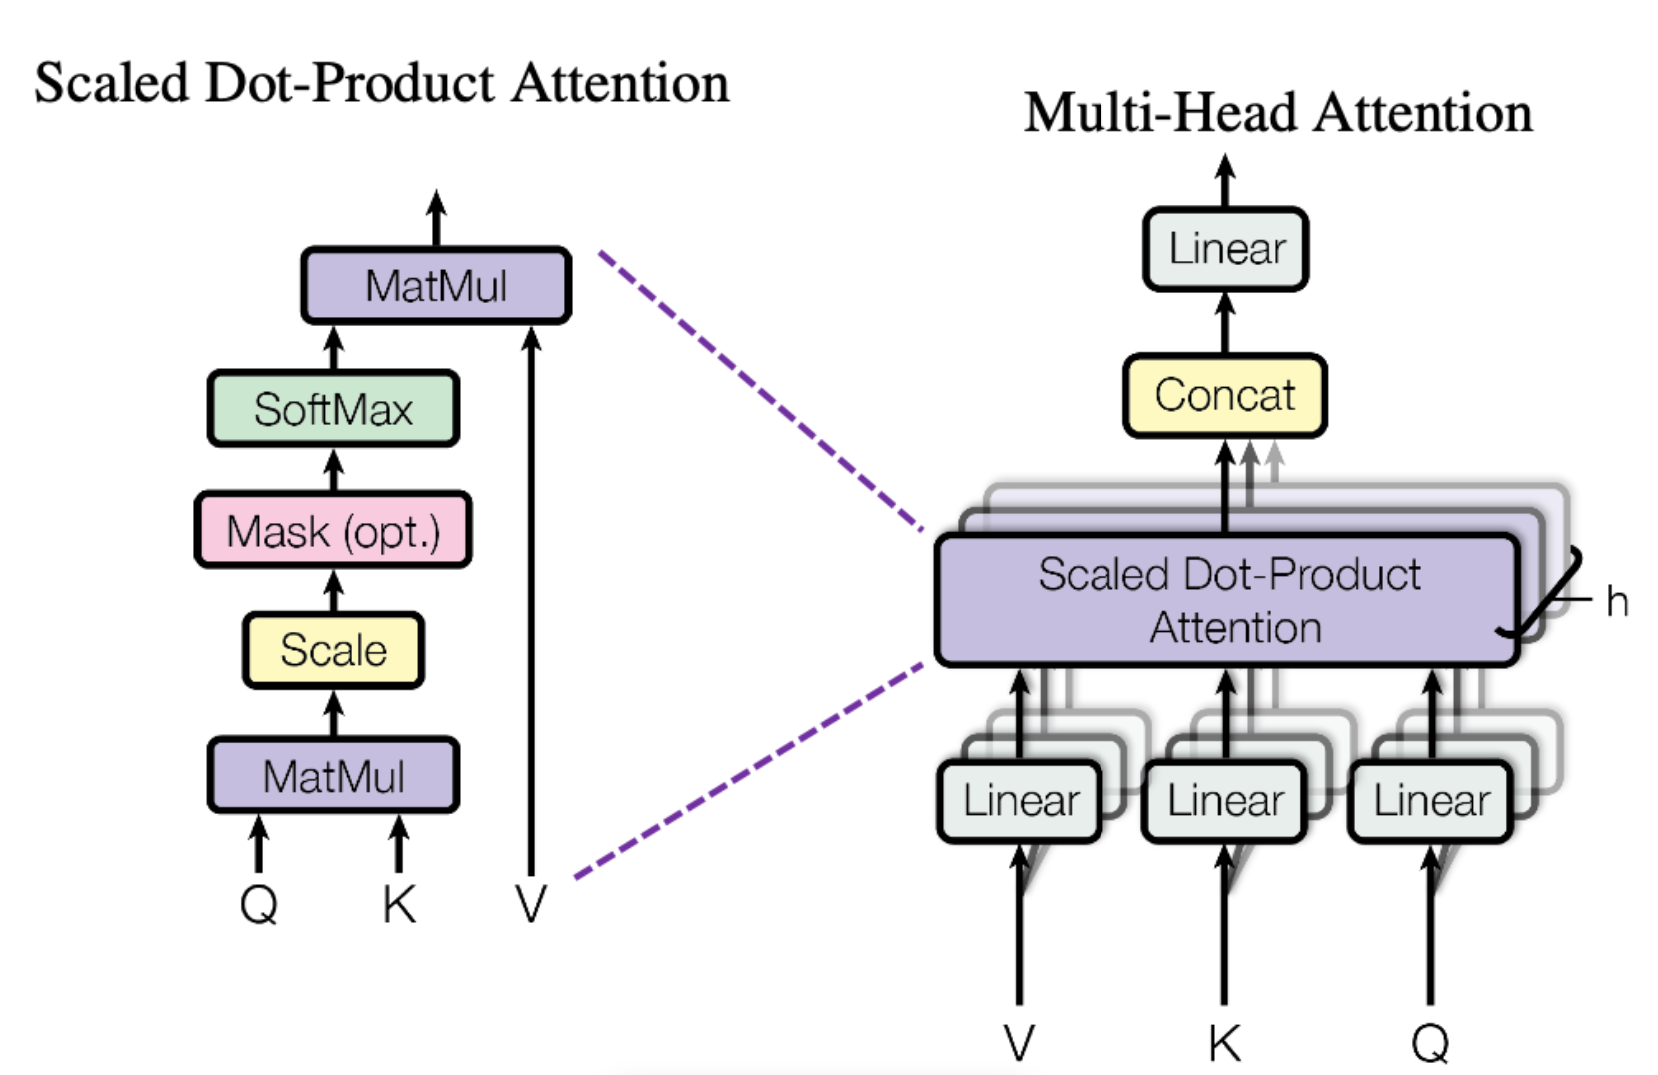
\includegraphics[width=0.7\textwidth]{figs/multihead_attn_1.png}}
%         \caption{توجه چندسر و توجه مقیاس‌شده بر پایه ضرب داخلی}
%         \label{fig:multihead_attn_1}
%     \end{figure}

%     در مرحله‌ی اول، بردار کلمات با گذر از سه لایه‌ی پیش‌خور 
%     (\lr{feed-forward layer})
%     با وزن‌های متفاوت، وکتورهای 
%     \lr{K}، \lr{V} و \lr{Q} 
%     را می‌سازند. سپس این وکتورها، وارد بلوک توجه مقیاس‌شده‌ی بر پایه‌ی ضرب داخلی
%     (\lr{Scaled Dot-Product Attention})
%     می‌شوند. در این بخش، ابتدا ضرب داخلی وکتورهای 
%     \lr{Q} و \lr{K} 
%     محاسبه می‌شود تا مشخص شود این دو چقدر به هم شبیهند.
%     سپس، با تقسیم امتیاز حاصل بر جذر طول رشته‌ی ورودی، 
%     امتیاز نرمال می‌شود تا از بروز مشکل انفجار گرادیان جلوگیری شود.
%     سپس، با اعمال تابع 
%     \lr{softmax}
%     بر روی این مقادیر، وزن هر کدام از کلیدها برای هر پرسش 
%     (\lr{query}) 
%     تعیین می‌شود. در نهایت، وزن‌های محاسبه‌شده در مقدارهای 
%     (\lr{value})
%     کلمات متفاوت ضرب می‌شوند تا خروجی مورد نظر تولید شود. 
%     این مراحل را می‌توانید در تصویر
%     \ref{fig:multihead_attn_1}
%     مشاهده کنید.
%     با توجه به این که کدگشا رشته‌ی خروجی را کلمه به کلمه تولید می‌کند،
%     باید درنظر داشته باشیم که وزن‌های توجه به گونه‌ای نباشند که کلمات به
%     واژه‌های بعد از خود توجه داشته باشند.

%     برای این کار، در روند توجه مقیاس‌شده‌ی بر پایه‌ی ضرب داخلی 
%     (\lr{Scaled Dot-Product Attention})
%     ، بعد از نرمال شدن امتیازها و قبل از اعمال تابع 
%     \lr{softmax}
%     ، آن‌ را با یک ماتریس اکیدا
%     بالا مثلثی که مقادیر بالای قطر اصلی آن منفی بی‌نهایت هستند جمع می‌کنیم.
%     این کار باعث می‌شود که بعد از اعمال تابع 
%     \lr{softmax}
%     ، مقدار وزن توجه هر کلمه به کلمه‌های بعد از خودش صفر شود. نمونه‌ای 
%     از این عمل سرپوش گذاری را می‌توانید در معادله
%     \ref{eq:22}
%     مشاهده کنید. 

%     \begin{center}
%         \begin{equation} \label{eq:22}
%            \begin{bmatrix}
%                 0.7 & 0.1 & 0.1 & 0.1 \\
%                 0.1 & 0.6 & 0.2 & 0.1 \\
%                 0.1 & 0.2 & 0.6 & 0.1 \\
%                 0.1 & 0.3 & 0.3 & 0.3
%            \end{bmatrix}
%             +
%             \begin{bmatrix}
%                 0 & -inf & -inf & -inf \\
%                 0 & 0 &  -inf & -inf \\
%                 0 & 0 &  0 &   -inf\\
%                 0 & 0 &  0 & 0
%            \end{bmatrix} 
%            =
%            \begin{bmatrix}
%             0.7 & -inf & -inf & -inf \\
%             0.1 & 0.6 &  -inf & -inf \\
%             0.1 & 0.2 &  0.6 &   -inf\\
%             0.1 & 0.3 &  0.3 & 0.3
%        \end{bmatrix} 
%         \end{equation}
%     \end{center}
% }
% \section{
%     مدل‌های زبان و تصویر بر پایه 
%     \lr{BERT}
% }
% \label{sec:bertlike_arcs}
% \paragraph{}
% {
%     مدل‌‌های تصویر و زبان خیرا شهرت بسیاری پیدا کرده‌اند. بر اساس وظیفه اعمال شده، 
%     معماری‌های متفاوتی برای حل مسائل تصویر و زبان در کنار یکدیگر ارائه شده است.
%     ر آنجایی که تبدیل کنندگان در بسیاری از موارد به خوبی عمل کردند، استفاده
%     از آن‌ها برای حل این مسائل اجنتاب‌ناپذیر است. بسیاری از این مدل‌های رائه‌شده
%     برپایه 
%     \lr{BERT}
%     یا معماریی مشابه با آن دارند. به طور کلی می‌توان این مدل‌ها را در دو دسته جای داد.
% }
% \subsection{
%     مدل‌های تک‌جریان
% }
% \label{subsec:single-stream-models}
% \paragraph{}
% {
%     معماری‌هایی هستند که هر دو بخش تصویر و زبان را در یک ماژول کدگذاری می‌شوند. 
%     همانطوری که در تصویر 
%     \ref{fig:single_stream}
%     مشخص است، بردار‌های تصویر و زبان هردو از یک ماژول تبدیل کننده عبور می‌کنند. 
%     مدل‌های تک‌جریان از لحاظ تعداد پارامترها بهینه هستند و از ابتدا به صورت 
%     تلفیقی بین بردار‌های تعبیه تصاویر و زبانی تناظر ایجاد می‌کنند.
%     \begin{figure}[H]
%         \center{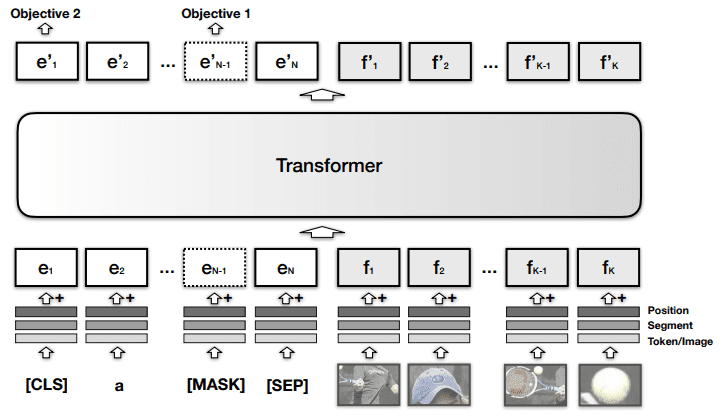
\includegraphics[width=0.6\textwidth]{figs/single_stream_arc.png}}
%         \caption{نمونه‌ای از یک مدل تک‌جریان}
%         \label{fig:single_stream}
%     \end{figure}
% }

% \subsection{
%     مدل‌های دوجریان
% }
% \label{subsec:dual-stream-models}
% \paragraph{}
% {
%     معماری‌هایی هستند که بخش تصویر و زبان در ماژول‌های جداگانه پردازش می‌شوند و 
%     سپس توسط ماژول دیگری ارتباط بین بردار‌های تعبیه شده زبانی با بردارهای 
%     تصویر را محاسبه می‌کند. 
%     با توجه به تصویر
%     \ref{fig:dual_stream}
%     هر دو بخش تصویر و زبان جداگانه جریان پیدا می‌کنند و سپس
%     یک تناظر بین این دو جریان بدست می‌آوریم. 
%     \begin{figure}[H]
%         \center{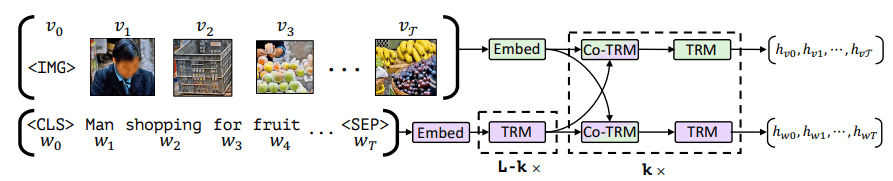
\includegraphics[width=1\textwidth]{figs/dual_stream_arc.png}}
%         \caption{نمونه‌ای از یک مدل دوجریان}
%         \label{fig:dual_stream}
%     \end{figure}
% }


\section{جمع‌بندی}
\paragraph{}
{
    در این فصل به شرح مفاهیم پایه‌ای پرداخته شد که در مراحل مختلف انجام
    این پژوهش مورد استفاده قرار گرفته و برای درک کامل خواننده‌ی
    این نوشتار مورد نیاز است.
    دراین فصل معماری‌ها و مدل‌های استفاده شده در این پزوهش به صورت جزیی مورد بررسی قرار
    گرفت. سپس به معرفی انواع مدل‌های موجود برای حل مسائل تصویر و زبانی پرداخته‌شد. 
    TODO
}
